\section{Messung der Spin-Relaxationszeit nach Dehmelt}
\label{sect:dehmelt}
\subsection{Durchführung}
Bei dieser Methode der Bestimmung der Spin-Relaxationszeit wird die Tatsache ausgenutzt,
dass bei Beleuchtung des Ensembles der Rubidiumatome durch \textsigma$^+$-Licht
zwei konkurrierende Prozesse vorliegen, die den Orientierungsprozess der Spins und damit
die Lichttransmission durch das Ensemble beeinflussen:
Zum einen findet eine Polarisation durch den Pumpprozess statt,
zum anderen eine Depolarisation (Relaxation).
Eine Variation der Stärke des Pumpprozesses durch Veränderung der Intensität des Laserlichts
erlaubt einen Rückschluss auf den konstant bleibenden Anteil der Relaxationsrate.

Während der Messung befinden sich die beiden Linsen und das \textlambda/4-Plättchen im Strahlengang,
sowie optional ein Neutraldichtefilter.
Das vertikale Erdmagnetfeld wird mit einem Strom von 93\,mA durch Spule~4 kompensiert.
Spule~3 erzeugt ein magnetisches Wechselfeld in Richtung des Laserstrahls,
das zweimal pro Periode eine Neuorientierung des Ensembles verursacht.
Verwendet wird dazu der \emph{instec function~generator},
die Frequenz des Rechtecksignals beträgt 50\,Hz und die Amplitude (Spitze-Spitze) 0.1\,V.

Das Absorptionssignal der Zelle wird am Oszilloskop erst mit 100\% Beleuchtungsintensität gemessen
und anschließend mit sieben verschiedenen Intensitäten (zwischen 2\% und 40\%),
die durch unterschiedliche Abschwächungen mit ND-Filtern im Strahlengang erreicht werden.

Die Temperatur des Lasers beträgt bei der Messung 34.0$^\circ$C, der Laserstrom 65.5\,mA
(sodass auf den beiden kurzwelligen Hyperfeinlinien von \rb{85} gepumpt wird).
Kurz vor der Aufnahme des Transmissionssignals wird die Rubidiumzelle mit dem Föhn geheizt.






\subsubsection*{Kalibrierung der Neutraldichtefilter}
Um die Stärke der verschiedenen Neutraldichtefilter festzustellen,
wird eine Kalibrierung mit Laser und Photodiode durchgeführt.
Die Temperatur des Lasers beträgt dabei 34.0$^\circ$C, der Laserstrom 52.0\,mA.
Die Spannung an der Photodiode wird ohne Filter gemessen und anschließend für zehn verschiedene Graufilter
mit nominellen Transmissivitäten von 0.001\% bis 50\%.
Ein weiterer Messpunkt wird mit ausgeschaltetem Laser aufgenommen.


\subsection{Auswertung}

\subsubsection*{Kalibrierung der Neutraldichtefilter}

\autoref{tab:deh:dnfilter} zeigt die Ergebnisse der Kalibrierung der Neutraldichtefilter:
Die Messwerte weichen stark von den nominellen Werten ab.
Zur Berechnung der transmittierten Intensität $I_\text{mess}$ wird
die an der Photodiode gemessene Spannung $U_{\text{ph}}$
durch die Spannung bei 100\% Intensität $U_{100}$ geteilt.
Beide Spannungen werden um die Offsetspannung $U_{0}=\text{-}70\,$mV (Messung bei ausgeschaltetem Laser) korrigiert:
\begin{equation}
  I_\text{mess}=\frac{U_{\text{ph}}-U_{0}}{U_{100}-U_{0}}
\end{equation}
Die Berechnung des Fehlers auf $I_\text{mess}$ erfolgt mit Gauß'scher Fehlerfortpflanzung.


Für die Bestimmung der Relaxationszeit werden nur die ersten sieben Filter verwendet,
da bei den Übrigen die Intensität der Transmission nicht für eine Messung ausreicht.

%TODO Tabelle ND Filter einfügen ohne input und erste ohne Filter schreiben und letzte zeile  mit ausgeschaltetem laser
\begin{table}[H]
\caption{xxx}
\begin{center}
\begin{tabular}{|c|c|c|c|c|}
  \hline
  Stärke & $I_\text{nominell}$ & $U$ / V & $I_\text{mess}$ & $s_{I_\text{mess}}$ \\ \hline
  0.0 & 100.000 & 749 & 1.00000 & 0.00000 \\ \hline
  0.3 & 50.000 & 257 & 0.39927 & 0.00799 \\ \hline
  0.6 & 25.000 & 218 & 0.35165 & 0.00703 \\ \hline
  1.0 & 10.000 & 55 & 0.15263 & 0.00305 \\ \hline
  1.3 & 5.000 & 3 & 0.08913 & 0.00178 \\ \hline
  2.0 & 1.000 & -28 & 0.05128 & 0.00103 \\ \hline
  2.3 & 0.500 & -44 & 0.03175 & 0.00063 \\ \hline
  2.6 & 0.250 & -52 & 0.02198 & 0.00044 \\ \hline
  3.3 & 0.050 & -63 & 0.00855 & 0.00017 \\ \hline
  4.0 & 0.010 & -68 & 0.00244 & 0.00005 \\ \hline
  5.0 & 0.001 & -69 & 0.00122 & 0.00002 \\ \hline
\end{tabular}
\end{center}
\label{tab:deh:dnfilter}
\end{table}


\subsubsection*{Transmissionssignale der Zelle und Fit}
\autoref{img:deh:trans3} zeigt beispielhaft für eine der acht Messungen
die Spannung der Photodiode $U_{\text{ph}}$,
die bei periodischer Modulation des Magnetfelds am Oszilloskop gemessen wurde.
Sie ist proportional zur transmittierten Lichtintensität.
Der Fit erfolgt gemäß \autoref{eq:expabhorient} mit einer Exponentialfunktion:
\begin{equation}
  U_{\text{ph}}(t)=a - b \cdot e^{-\frac{t}{\tau}}
\end{equation}
Der Parameter $a$ beschreibt die Transmission im Gleichgewicht, $b$ die Amplitude der
Transmissionsänderung und $\tau$ die gesuchte Orientierungzeit des Ensembles.

\begin{figure}[H]
\begin{center}
  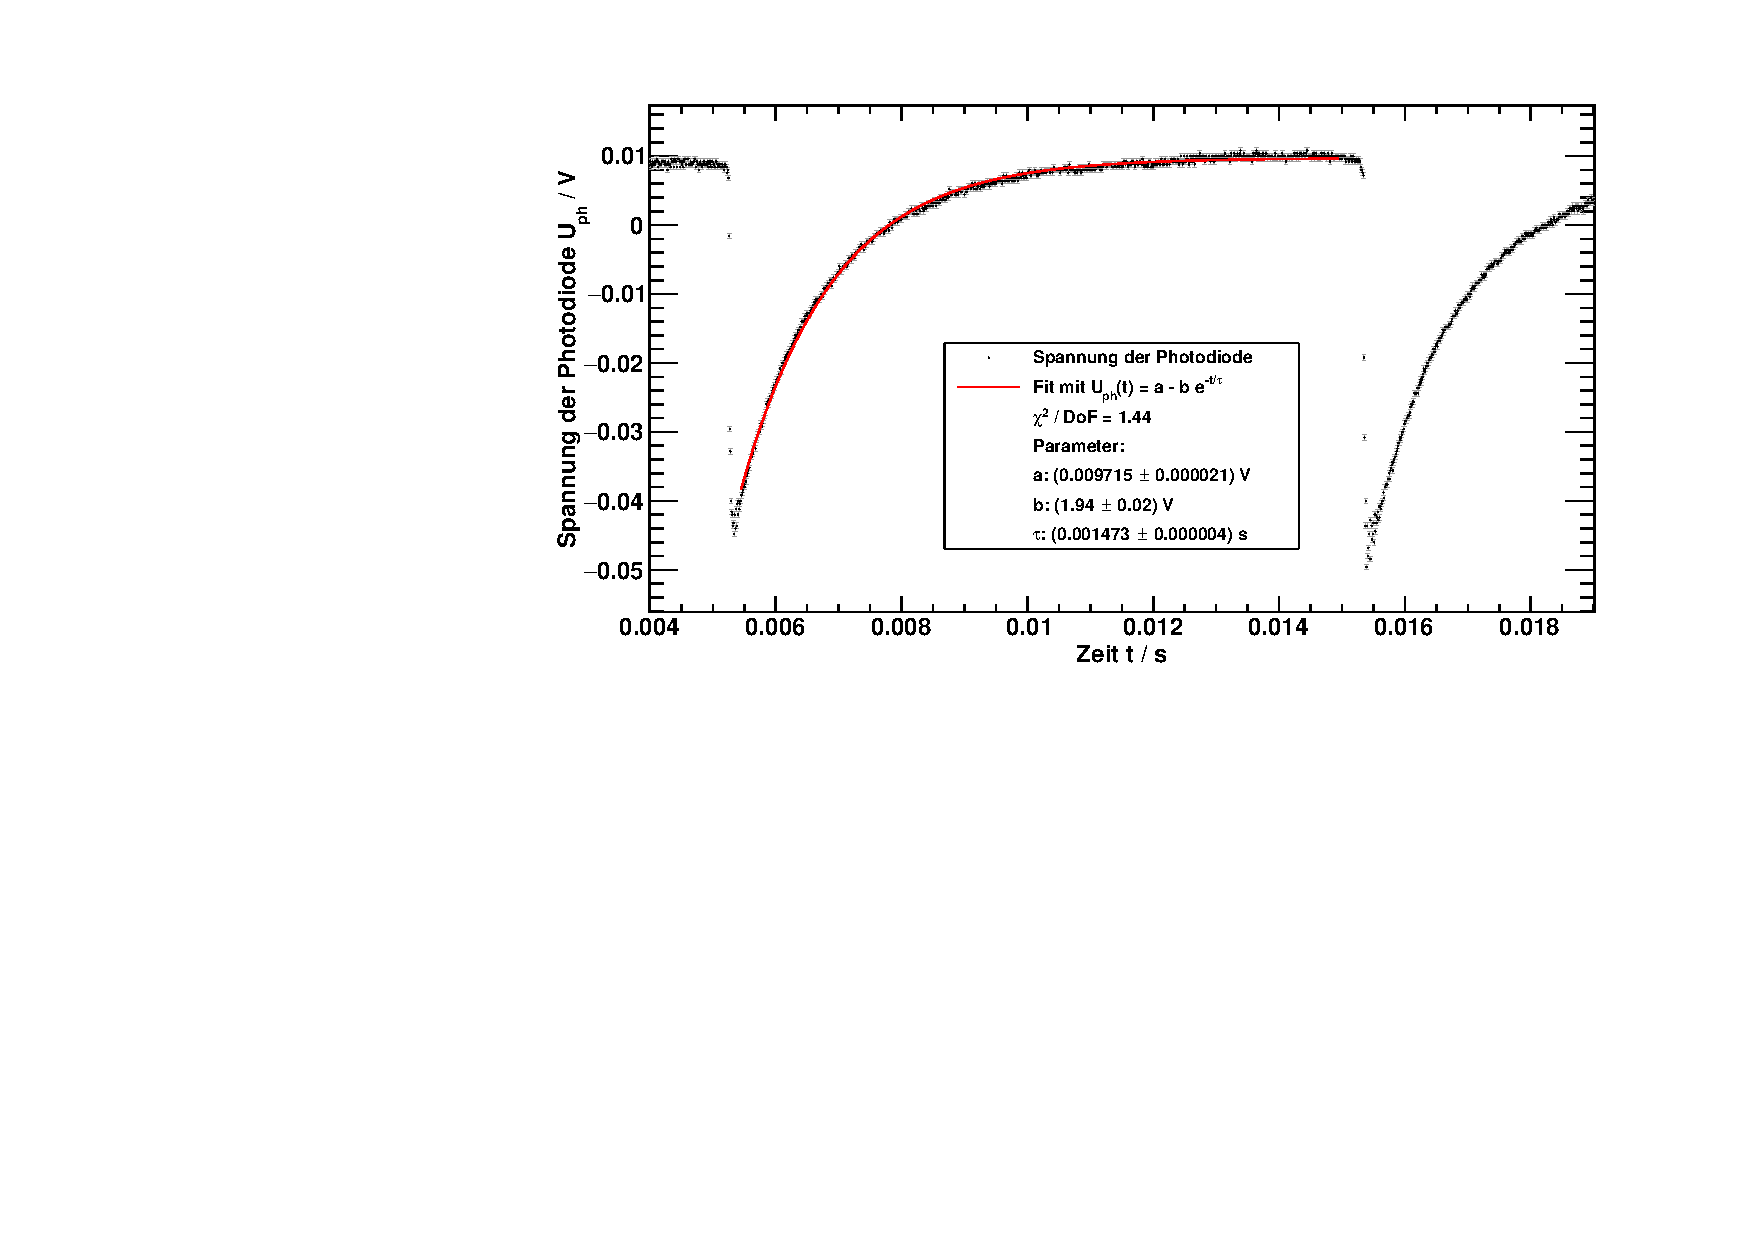
\includegraphics[width=\textwidth]{../img/part5/65-5mA-10.pdf}
  \caption{Beispiel einer Messung zur Bestimmung der Orientierungszeit des Rubidiumgases:
  Spannung der Photodiode (entspricht der Transmission durch die Rubidiumzelle)
  nach Umkehr des Magnetfelds.
  Die Anstiegszeit $\tau$ des Fits wird durch Polarisations- und Relaxationsprozesse bestimmt.}
  \label{img:deh:trans3}
\end{center}
\end{figure}


In \autoref{tab:part3:results} sind die Ergebnisse für die Anstiegszeiten $\tau$
der Fits an die acht Transmissionssignale aufgeführt.

%TODO Tabelle copy paste und geltende ziffern schön machen

\begin{table}[H]
\caption{xxx}
\begin{center}
\begin{tabular}{|c|c|c|c|}
  \hline
  $I$ & $s_I$ & $\tau$ / ms & $s_\tau$ / ms \\ \hline
  1.0000 & 0.0000 & 0.344 & 0.002 \\ \hline
  0.3993 & 0.0080 & 0.749 & 0.003 \\ \hline
  0.3516 & 0.0070 & 0.872 & 0.004 \\ \hline
  0.1526 & 0.0031 & 1.473 & 0.004 \\ \hline
  0.0891 & 0.0018 & 1.932 & 0.004 \\ \hline
  0.0513 & 0.0010 & 2.439 & 0.005 \\ \hline
  0.0317 & 0.0006 & 2.831 & 0.013 \\ \hline
  0.0220 & 0.0004 & 3.032 & 0.016 \\ \hline
\end{tabular}
\end{center}
\label{tab:deh:fitres}
\end{table}


\subsubsection*{Bestimmung der Relaxationszeit}
Um die Relaxationszeit $T_{\text{R}_\text{D}}$ zu bestimmen, also ihren Anteil aus den gemessenen Orientierungszeiten zu extrahieren,
wird \autoref{eq:orientierungszeit} benutzt sowie der Umstand,
dass die charakteristische Pumpzeit $T_\text{P}$ umgekehrt proportional zur Intensität $I$ des Laserlichts ist:
\begin{equation}
  T_\text{P} = \frac{1}{\alpha I} 
\end{equation}
Man erhält damit
\begin{equation}
  \frac{1}{\tau(I)}=\alpha I + \frac{1}{T_{\text{R}_\text{D}}} \ \,.
\end{equation}
Dieser Zusammenhang wird benutzt, um eine Kurvenanpassung an die Daten aus \autoref{tab:part3:results}
durchzuführen und die Relaxationszeit $T_{\text{R}_\text{D}}$ zu bestimmen.
\autoref{img:deh:relaxtime} zeigt diesen Fit an die inversen Orientierungszeiten.

\begin{figure}[H]
\begin{center}
  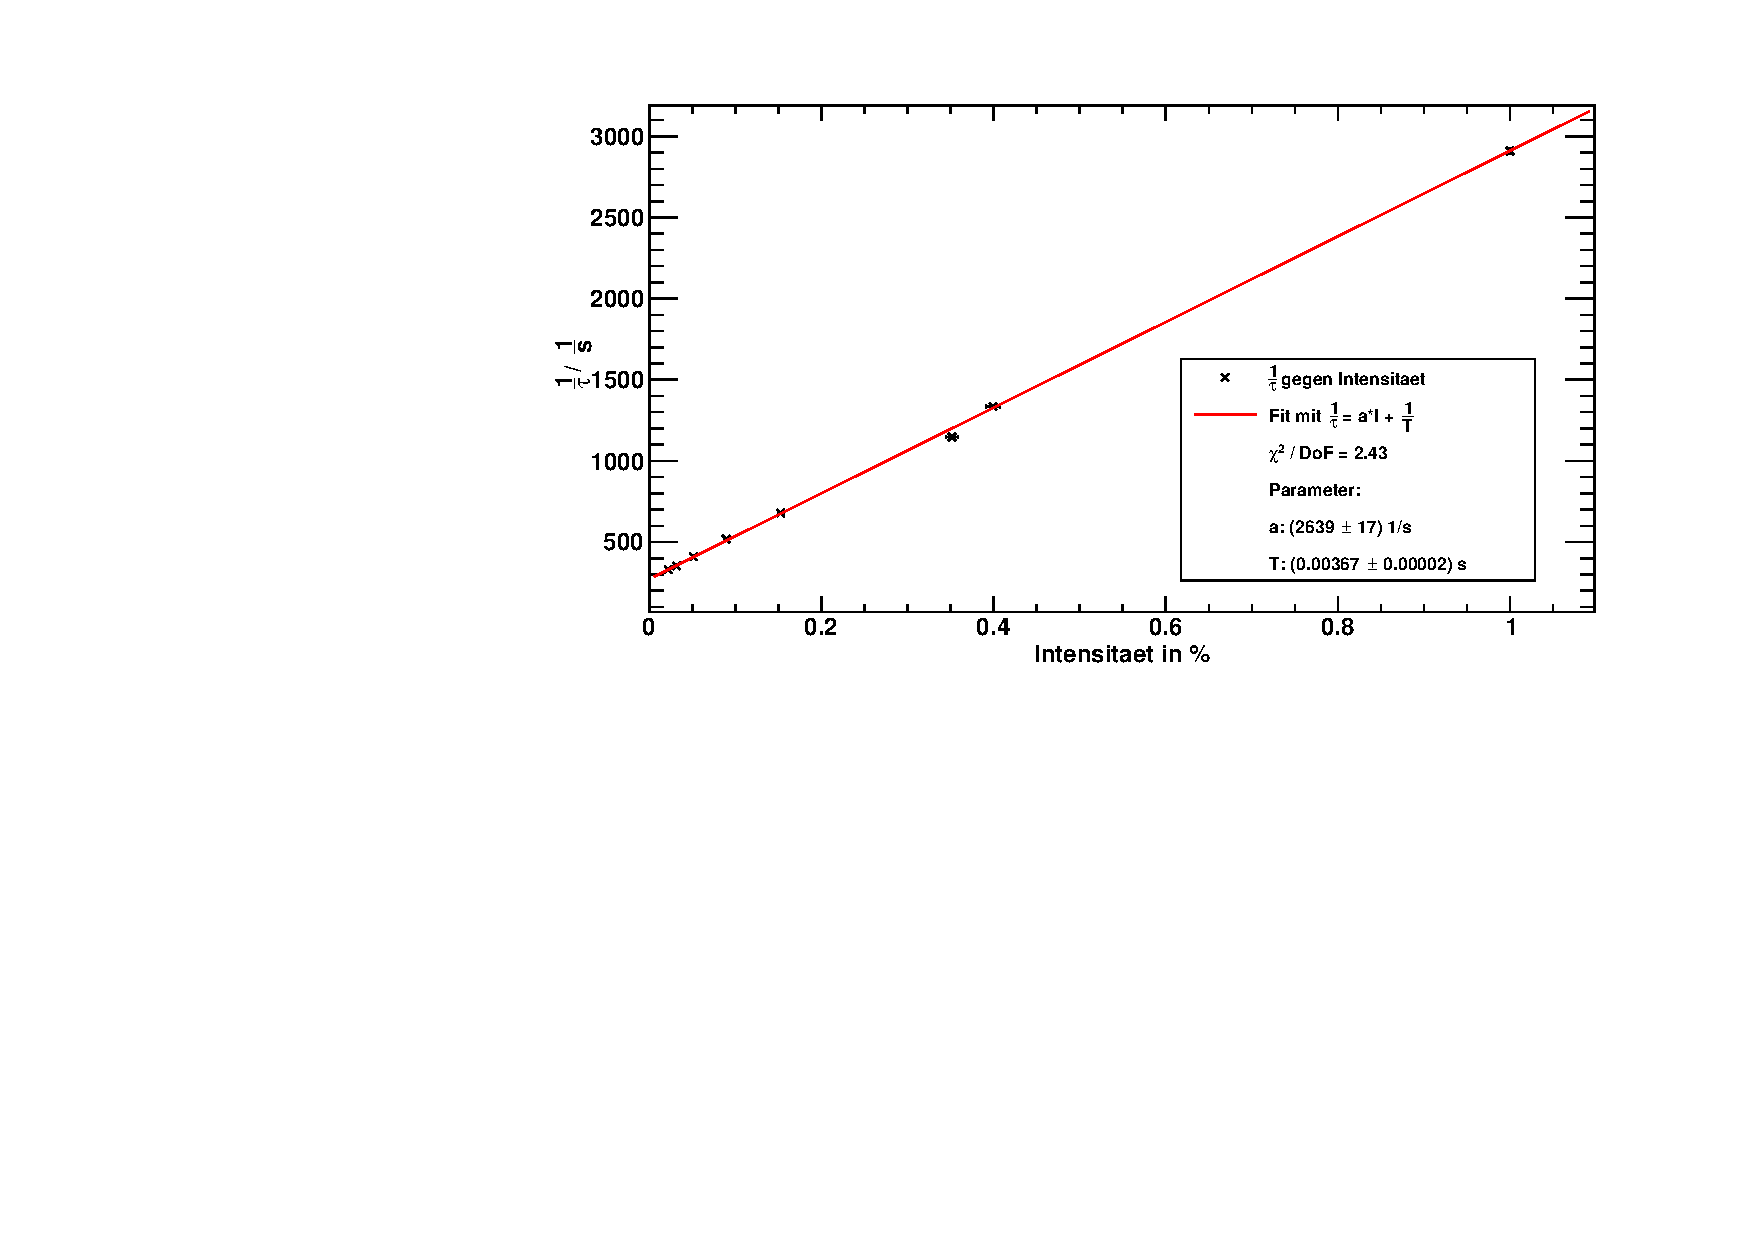
\includegraphics[width=\textwidth]{../img/part5/taufit.pdf}
  \caption{Lineare Kurvenanpassung an die Daten aus \autoref{tab:part3:results} zur Extraktion
  der Relaxationszeit $T_{\text{R}_\text{D}}$ aus den Messdaten für die Orientierungszeit~$\tau$.}
  \label{img:deh:relaxtime}
\end{center}
\end{figure}

Das Ergebnis für die Relaxationszeit beträgt
\begin{equation}
  T_{\text{R}_\text{D}} = 3.64 \pm 0.02\,\text{ms}
\end{equation}
und stimmt..
%TODO vgl litval Tr dehmelt



